\documentclass[a4paper]{amsart}
\usepackage[top=0.5cm,bottom=0.5cm,left=0.25cm,right=0.5cm]{geometry}
\usepackage{siunitx}
\usepackage{tikz}
\usetikzlibrary{calc}
\usepackage{pgfplots}
\pgfplotsset{compat=1.3}

\begin{document}
	\thispagestyle{empty}
	\begin{figure}
		\centering
		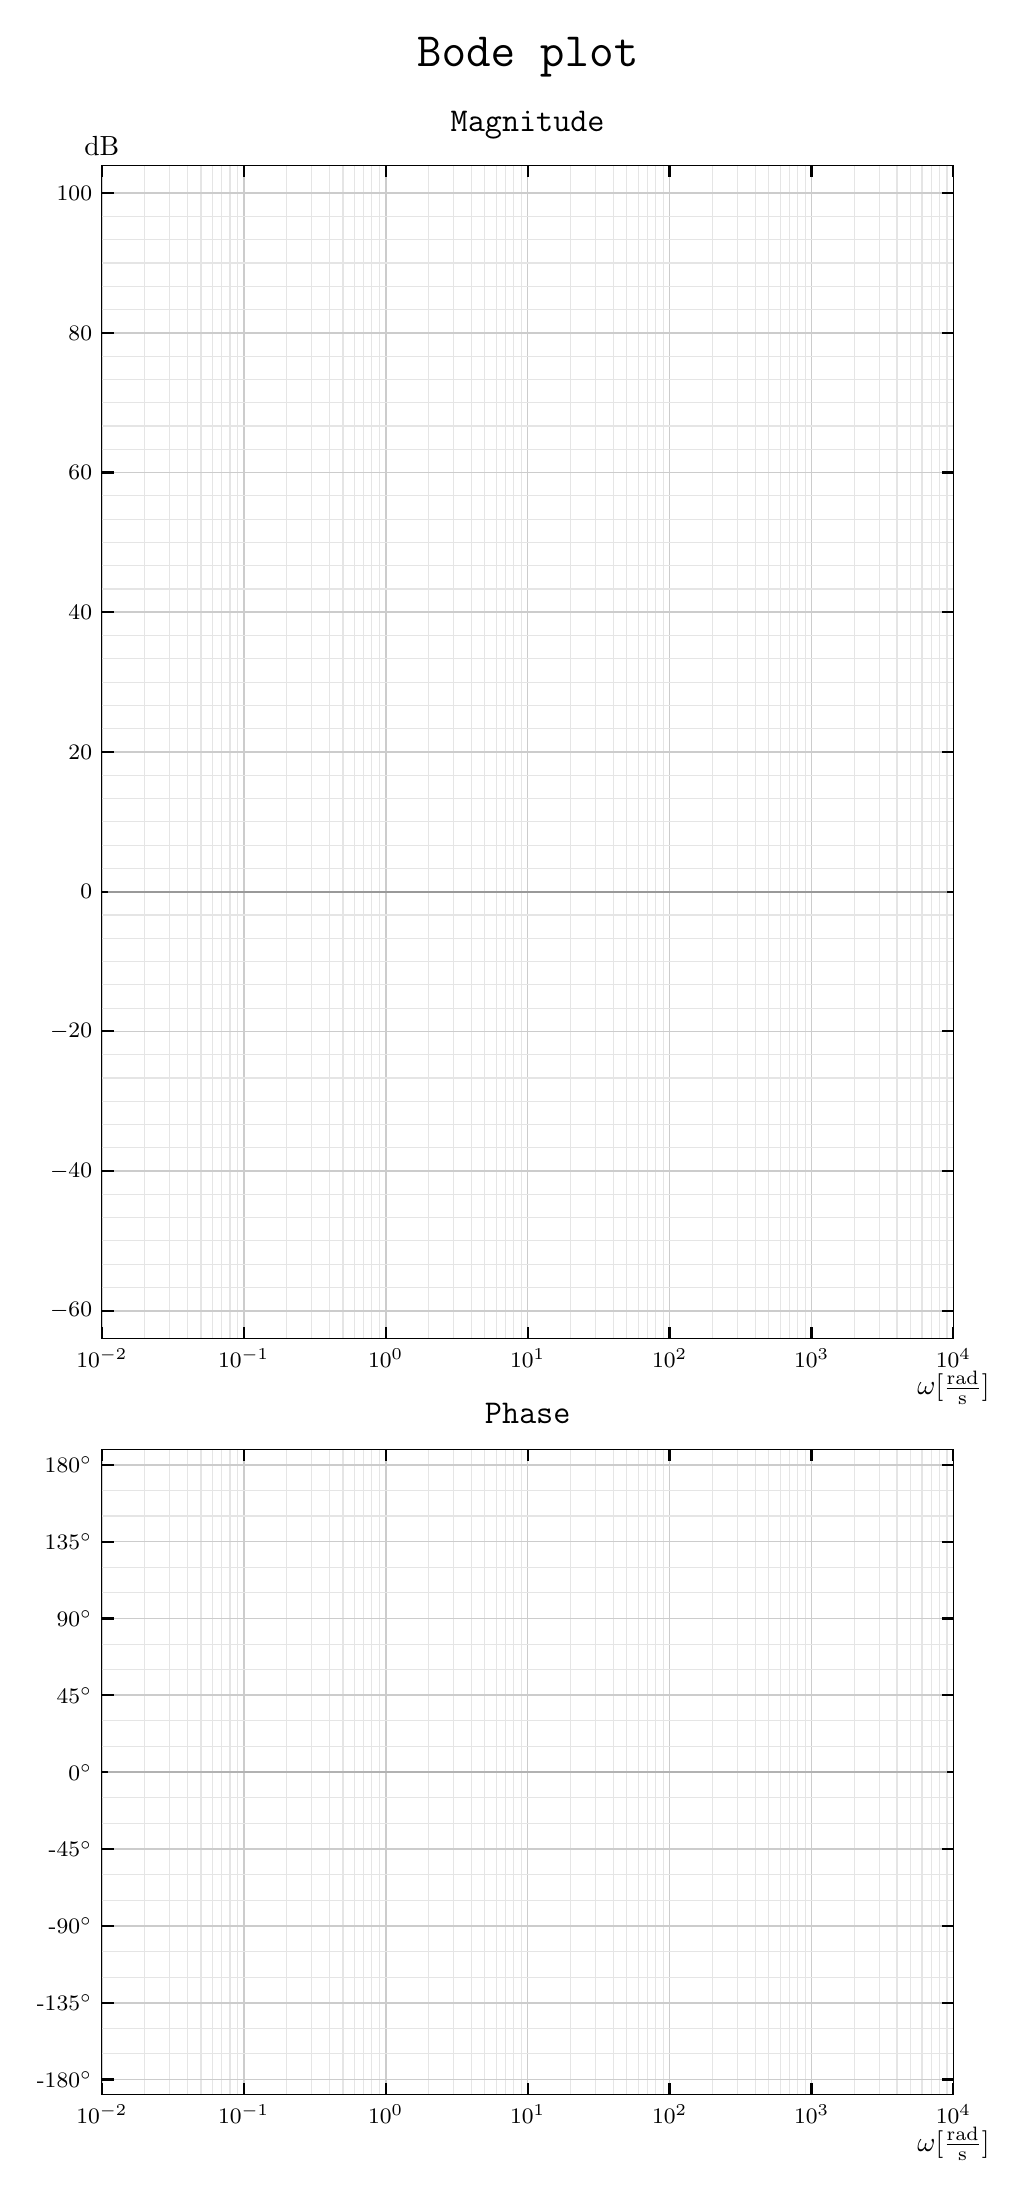
\begin{tikzpicture}
			\begin{axis}[
				name=magnitude,
				title={\texttt{\large{Magnitude}}},
				width=1.0225\linewidth,
				height=0.59\paperheight,
				xmode=log,
				ymode=linear,
				axis line style={latex-latex},
				xlabel={$\omega$[\si[per-mode=fraction]{\radian\per\second}]},
				xlabel style={at={(ticklabel* cs:1,8)},anchor=north},
				ylabel={\si{\decibel}},
				ylabel style={rotate=-90,at={(ticklabel* cs:1)},anchor=south},
				xmin=1e-2,xmax=1e4,
				ymin=-60,ymax=100,
				enlarge y limits=0.025,
				ytick={-60,-40,...,100},
				grid=both,
				minor tick num=5,
				grid style={line width=.4pt, draw=gray!20},
				minor tick style={line width=.4pt, draw=gray!20},
				major tick style={line width=.8pt,draw=black},
				major grid style={line width=.6pt,draw=gray!40},
				ticklabel style={font=\footnotesize}
			]
			\addplot[mark=none,line width=.8pt,gray!80,domain=0.011:9000]{0}; % Makes "0 axis" thicker
			\end{axis}
			\begin{axis}[
				name=phase,
				title={\texttt{\large{Phase}}},
				at={($(magnitude.south)-(0,40)$)},
				anchor=north,
				width=1.0225\linewidth,
				height=0.35\paperheight,
				xmode=log,
				ymode=linear,
				axis line style={latex-latex},
				xlabel={$\omega$[\si[per-mode=fraction]{\radian\per\second}]},
				xlabel style={at={(ticklabel* cs:1,8)},anchor=north},
				xmin=1e-2,xmax=1e4,
				ymin=-180,ymax=180,
				enlarge y limits=0.025,
				ytick={-180,-135,...,180},
				yticklabels={-180$^\circ$,-135$^\circ$,-90$^\circ$,-45$^\circ$,0$^\circ$,45$^\circ$,90$^\circ$,135$^\circ$,180$^\circ$},
				grid=both,
				minor tick num=2,
				grid style={line width=.4pt, draw=gray!20},
				minor tick style={line width=.4pt, draw=gray!20},
				major tick style={line width=.8pt,draw=black},
				major grid style={line width=.6pt,draw=gray!40},
				ticklabel style={font=\footnotesize}
			]
			\addplot[mark=none,line width=.8pt,gray!60,domain=0.011:9000]{0};
			\end{axis}
			\node[above,font=\large\bfseries] at ($(magnitude.north)+(0,1)$) {\texttt{\LARGE{Bode plot}}};
		\end{tikzpicture}		
	\end{figure}
\end{document}